\chapter{Compiling exceptions totally correctly}

\todo{Blah blah about differences between FP and total FP, substantiate the
title of the section}

The basic approach to compiling exceptions was shown in \cite{gmh:exceptions}.
This article provides excellent insight and inspiration how such code can be written
in a language such as Haskell.
However, peculiarities of programming with dependent types will make us
diverge a bit, in details at first, in parts of the design later.
\todo{The above is not completely true, FIXME.}

\section{Adding exceptions, GMH-style}

Now we are about to add exceptions to our language(s). The first approach is to
examine the ways found in the literature.

Code in this section is modelled after the paper \cite{gmh:exceptions} by
Graham Hutton and Joel Wright. The authors used Haskell in their development.
This approach was later formalized by Tobias Nipkow in \cite{nipkow} in
Isabelle, an interactive theorem prover/proof assistant, in exactly the same
way; the development even uses the same lemmas and their numbering as the
paper.

In contrast with the original paper and Tobias Nipkow's formalization thereof,
our aim is to create a dependently typed program, which means we don't want to
copy the Haskell code as is; instead, we will adapt it for the dependently
typed setting and see how it works out.

\subsection{Changes to the high-level language}

\subsubsection{Expressions}

The first module we need to extend when adding exceptions is the one containing
the definition of expressions of the high-level language. Namely, we need to
add the \ident{Throw} expression and the \ident{Catch} construct.

\begin{code}
  data Op : U -> U -> U -> Set where
    Plus : Op nat nat nat
\end{code}

\begin{code}
  data Exp : U -> Set where
    Lit : forall {u} -> el u -> Exp u
    Bin : forall {u v w} -> Op u v w -> Exp u -> Exp v -> Exp w
    Throw : forall {u} -> Exp u
    Catch : forall {u} -> (val : Exp u) -> (hnd : Exp u) -> Exp u
\end{code}

\noindent The type of expressions gets two new constructors.
\begin{itemize}

  \item One of them is \ident{Throw}, which is similar to the literal
    constructor \ident{Lit}, except that no value of the type \ident{el u} is
    needed: a throw-expression can promise to yield a value of any type without
    actually having it.

  \item The other one is \ident{Catch}. This constructor takes two expressions of
    the same type, the regular value and an exception handler, representing a
    catch-block.

\end{itemize}

\subsubsection{Semantics of expressions}

The expression type has just been extended with two new constructors and we
need to formalize what the meaning of the two expression variants actually is.
For that purpose, we need to alter the function \ident{denExp}.

The first change is in the return type of \ident{denExp}: we need a way to
indicate whether the expression evaluates to a value or whether an uncaught
exception occurs. To express that, the function \ident{denExp} will now return
\ident{Maybe (el u)} instead of the more direct \ident{el u}, using the value
\ident{nothing}\footnote{In contrast with Haskell, Agda uses lowercase initials
of the constructors \ident{just} and \ident{nothing}.} to indicate uncaught
exceptions and the value \ident{just x} to indicate that the expression
succesfully evaluates to the value~\ident{x}.

The second change is adding pattern cases for the newly added constructors
of \ident{Exp} to the denotation function \ident{denExp}.

\begin{code}
  denExp : forall {u} -> Exp u -> Maybe (el u)
  denExp (Lit x) = just x
  denExp (Bin op l r) with denExp l | denExp r
  \... | just x  | just y  = denOp op x y
  \... | just _  | nothing = nothing
  \... | nothing | just _  = nothing
  \... | nothing | nothing = nothing
  denExp Throw = nothing
  denExp (Catch e h) with denExp e
  \... | just x  = just x
  \... | nothing = denExp h 
\end{code}

\noindent We had to alter the original two cases slightly, most importantly the
binary operator case, where the result now yields a value (i.e.  doesn't throw)
if and only if both subexpressions yield values without throwing.

As hinted above, we added a case for the expression \ident{Throw}: this one
never yields a value and always throws; and also case for catch-expressions: if
no exception gets thrown in the value, the whole catch-expression is equivalent
to the regular value.  Otherwise, it is equivalent to the handler
value.\footnote{Especially, if both values throw exceptions, the
catch-expression propagates the exception thrown in the handler.}
\footnote{Hence, this constructor is similar to the combinator \ident{mplus} in
Haskell, which combines two possibly failing computations in exactly the same
way.}

\subsubsection{Remarks}

To keep things simple, the \ident{Throw} expression does not take a value,
unlike its counterparts in most programming languages. At this stage, we will
worry only about whether an exception has been thrown or not, not about its
particular value.

Also, in most programming languages, exception handlers can inspect the
exceptions being handled and return different values depending on some
attributes of the exception. In our language, it would be pointless to do that
because our exceptions do not carry values. Thus, our exception handlers are
just simple expressions of the same type as the main expression and they have
no means to refer to the exception being handled.

This concludes the definition of our high-level language and the rest of this thesis
will be mostly devoted to how to make it work operationally.

\subsection{Virtual machine}

What about our virtual stack machine and its low-level language of
instructions? What features and instructions do we need to add to make the
machine capable of computing with exceptions?

In \cite{gmh:exceptions}, Hutton and Wright give a description of how this can
be done. Let us extend the machine along the lines drawn by this paper and see
how we can adapt their solution to total functional programming with dependent
types, having the goals from the Introduction (page~\pageref{objectives}) in
mind.

\subsubsection{Stack}

First, Hutton and Wright propose altering the type of stacks because besides
values, now we are going to push exception handlers on the stack, too.

Unlike Hutton and Wright, we also need to care about stack shapes.
The type of stack shapes will no longer be a plain
list of types (that is, elements of the universe~\ident{U}); instead, we  will
distinguish between \emph{values} and \emph{handlers} pushed on the stack.
\footnote{Actually, there is even more ``dependent'' approach: we could
index the type of stack shapes by the list of handlers on the stack, getting
\ident{Shape : List U $\to$ Set}. In this setup, pushing a value on the stack
will change its shape but not the type of the shape, while pushing a handler
on the stack will change both the shape and the type of the shape. However, we
will not take this route as it turns out to be more complicated, while the author
could not see any advantages this would yield.}

\begin{code}
  data Item : Set where
    Val : U -> Item
    Han : U -> Item

  Shape : Set
  Shape = List Item
\end{code}
A value, denoted by \ident{Val u}, is an actual value of the type
denoted by \ident{u}; a handler, denoted by \ident{Han u}, is a piece of code
that, when run, leaves a value of the type \ident{u} on the top of the stack.
This naturally leads to the new type of stacks,
\label{sec:gmh-ham-stack}\begin{code}
  data Stack : Shape -> Set where
    snil : Stack []
    _\scons\_ : forall {u s} -> el u -> Stack s -> Stack (Val u :: s)
    _\sconsh\_ : forall {u s} -> Code s (Val u :: s) -> Stack s -> Stack (Han u :: s)
\end{code}
where the constructor \ident{\scons\!\!} corresponds to pushing values and the
constructor \ident{\sconsh\!\!} corresponds to pushing handlers on the stack.

Note that we push arbitrarily large strands of code as single items on the stack,
which contradicts one of our design principles -- that the
code must be executable on a simple stack machine (Introduction, page~\pageref{objectives})
-- and we will address this objection in \Fref{chap:compiling2}.

\subsubsection{Instructions and code}

Next, Hutton and Wright introduce three new instructions of the virtual machine:
\ident{MARK}, \ident{UNMARK}, and \ident{THROW}. In our code, this change
reflects in extending the \ident{Instr} type, which must now reside in a
\ident{mutual} block with \ident{Code}:

\label{sec:gmh-ham-instr}\begin{code}
  mutual
    data Instr : Shape -> Shape -> Set where
      PUSH : forall {u s} -> el u -> Instr s (Val u :: s)
      ADD : forall s -> Instr (Val nat :: Val nat :: s) (Val nat :: s)
      THROW : forall {u s} -> Instr s (Val u :: s)
      MARK : forall {u s} -> Code s (Val u :: s) -> Instr s (Han u :: s)
      UNMARK : forall {u s} -> Instr (Val u :: Han u :: s) (Val u :: s)

    Code : Shape -> Shape -> Set
    Code = Star Instr
\end{code}

\noindent The definition of code doesn't change: it is still a simple
``index-matching list'' of instructions.

\subsubsection{Compiler}

We will first use the compiler presented by Hutton and Wright in
\cite{gmh:exceptions}, studying how execution can be implemented in a
dependently typed setting.

The general idea is that before evaluating a (sub-)expression, we push
the corresponding exception handler on the stack, if available. After
successful execution of the corresponding code, the handler is removed
from the stack.

This compiler is quite similar to the one we introduced for simple
exceptionless expressions in \Fref{sec:simple-compiler}. We will keep all
definitions: the functions $[\!\![\_]\!\!]$ and \ident{opInstr}, and both cases
of the function \ident{compile} -- these will be just extended with two new
clauses for the expressions \ident{Throw} and \ident{Catch}.

\label{sec:gmh-ham-compile}\begin{code}
compile : forall {u s} -> Exp u -> Code s (Val u :: s)
compile (Lit x) = [[ PUSH x ]]
compile (Bin op l r) = compile r \app compile l \app [[ opInstr op ]] 
compile Throw = [[ THROW ]]
compile (Catch e h) = [[ MARK (compile h) ]] \app compile e \app [[ UNMARK ]]
\end{code}

The expression \ident{Throw} compiles to a single \ident{THROW} instruction;
the expression \ident{Catch} generates a \ident{MARK}-\ident{UNMARK}-delimited
block containing the \emph{guarded expression} and the associated handler.

\section{Execution: placeholders}

\subsection{Machine state}

The topic of machine state is left implicit in the paper by Hutton and Wright,
yet it is one of the most involved parts of this Agda development. We have to
make it completely explicit in order to adhere to our objectives.

To put it precisely, the state of the virtual machine includes
the following components:
\begin{itemize}
	\item the position in the executed code (``instruction pointer'');
	\item the stack;
	\item a bounded number of other flags and variables.
\end{itemize}

Then, execution is fully specified if for each instruction, we define its
effect on the machine state.

For now, we will leave the position in the code implicit and we will not count
it as a component of the state. The motivation for doing so is retaining
the ability to recurse over code structurally, which we would lose if we
permitted any manipulation with code (beyond un-consing done by the execution
function).

\subsection{Placeholder method}

One approach\footnote{This approach is not considered by Hutton and Wright at all;
we include it for illustration as the most na\"{i}ve strategy, whose disadvantages
will be gradually solved as we will be switching to better and better approaches.}
to execution not requiring any additional flags and variables
would be extending the stack type with a new constructor; let us call it
\ident{\void\scons\!\!\_}.
\begin{code}
  data Stack : Shape -> Set where
    snil : Stack []
    _\scons\_ : forall {u s} -> el u -> Stack s -> Stack (Val u :: s)
    _\sconsh\_ : forall {u s} -> Code s (Val u :: s) -> Stack s -> Stack (Han u :: s)
    \void\scons\_ : forall {u s} -> Stack s -> Stack (Val u :: s)
\end{code}
The new constructor acts as a placeholder for missing values if an exception is raised.

Note the strong similarity of the new constructor \ident{\void\scons\_} to the
\ident{THROW} instruction and the \ident{Throw}
expression. The instruction \ident{THROW} is indexed as an instruction that pushes
a value of any specified type on the stack -- but it actually does not. The 
\ident{Throw} expression is indexed as an expression that yields a value of any specified
type -- but it actually does not. Likewise, the \ident{\void} constructor is typed in
exactly the same way as the constructor that pushes values on the stack -- but it does not.

Thus, it is probably not a surprise that the \ident{THROW} instruction, instead of pushing
a value on the stack, pushes the \ident{\void} placeholder. To be precise, execution would
look the following way. \label{sec:placeholder}
\begin{code}
  mutual
    execInstr : forall {s t} -> Instr s t -> Stack s -> Stack t
    -- the original two cases
    execInstr (PUSH x) st = x \scons st
    execInstr ADD (x \scons y \scons st) = (x + y) \scons st
    -- new instructions
    execInstr THROW st = \void\scons st
    execInstr (MARK h) st = h \sconsh st
    -- unmark: no exceptions thrown
    execInstr UNMARK (x \scons h \sconsh st) = x \scons st
    -- unmark: an exception thrown, handle it by executing the handler
    execInstr UNMARK (\void\scons h \sconsh st) = execCode h st
    -- miscellaneous exception handling
    execInstr ADD (\void\scons y \scons st) = \void\scons st
    execInstr ADD (x \scons \void\scons st) = \void\scons st
    execInstr ADD (\void\scons \void\scons st) = \void\scons st

    -- execCode is still a left fold over instructions
    execCode : forall {s t} -> Code s t -> Stack s -> Stack t
    execCode \nil st = st
    execCode (i <| is) st = execCode is (execInstr i st)
\end{code}

\noindent However, there are multiple downsides to this solution.%
\label{sec:placeholders-objections}

First, and most importantly, it's not really a transition to a different
low-level language.  Instead, it is actually evaluation of the function
\ident{denExp} with an explicit stack. The placeholder \ident{\void}
corresponds to the outcome \ident{nothing} of \ident{denExp}, while the regular
stack-cons using the constructor \ident{\scons\!\!} corresponds to the outcome
\ident{just x} (for some \ident{x}).

Second, this solution is not elegant in the sense that we need to add
exception-handling cases to every instruction (in our case, only \ident{ADD}).
Why should we define how these instructions handle exceptions when they all
must do the same thing: just pass the exception forward and do nothing else?
Exceptions should be handled by a different mechanism than regular execution.

Third, this approach is also inefficient. Defining how single instructions
handle exceptions means that these instructions are going to be executed.
However, we can do better: simply skip the appropriate number of instructions
-- and real machines are good at skipping efficiently.

Fourth, the Agda termination checker rejects the exception-handling case for
\ident{UNMARK} in the function \ident{execInstr}. Recursion isn't structural
here and we need to convince Agda about termination using a decreasing measure
or another way.

Fifth, it is not how machines actually work. Apart from doing jumps, real-world
exception-handling strategies don't push whole code blobs on the stack.
Instead, they linearize exception-handling code with regular code into a single
instruction sequence -- and then they jump around as needed.

While this low-level representation does work, it leaves much to be desired. In
the following sections (and chapters), we will address these objections. Let us
begin with the first three of them.

\section{Execution: stack unwinding}

We will adapt the method of \emph{stack unwinding}, described in the paper by Hutton
and Wright. Now the machine will have two modes of execution, as hinted in
\cite[p.~7]{gmh:exceptions}.

The normal mode is exactly what one would expect: executing instructions on a stack, nothing surprising.

However, the non-trivial part is the exception-handling mode. When an exception is thrown,
two things need to be done in order to execute the exception handler: \label{sec:stack-unwinding}
\begin{itemize}
	\item The stack needs to be unwound. This means removing items from the stack
		until the first exception handler.\footnote{Here we do not distinguish types
		of exception handlers so any handler is always appropriate. If we had typed
		exceptions, we might need to skip handlers that don't match the exception
		being processed.} When this is done, we can pop the handler from the stack
		and the resulting stack is now suitable for execution of the popped handler.
	\item The position in the sequence of instructions needs to be advanced
		appropriately. In general, we need to skip all instructions that belong
		to the computation being abandoned.
\end{itemize}

\subsection{Handler frames}
In a sense, we can talk about \emph{handler frames} that we need to discard
while looking for an exception handler. This is best demonstrated on an example.
Consider the following expression of the high-level language:
\begin{code}
  Bin Plus
  	(Catch
  		(Bin Plus (Lit 1) (Lit 4))
  		(Lit 2))
  	(Lit 3)
\end{code}
The above expression compiles to the following instruction sequence, where we use
the name~\ident{h} for the compiled handler code\footnote{In this case, the handler
code is \ident{[PUSH 2]}.} for readability.
\begin{code}
  [PUSH 3, MARK h, PUSH 4, PUSH 1, ADD, UNMARK, ADD]
\end{code}
This code does not throw any exceptions so we already know how it should be executed.
Let us plot the intermediate stacks in a graph, with the executed instructions
on the horizontal axis, and the stack growing vertically from the baseline. This is
how we get \Fref{fig:stack-frames}.

\begin{figure}[tp]
	\centering
	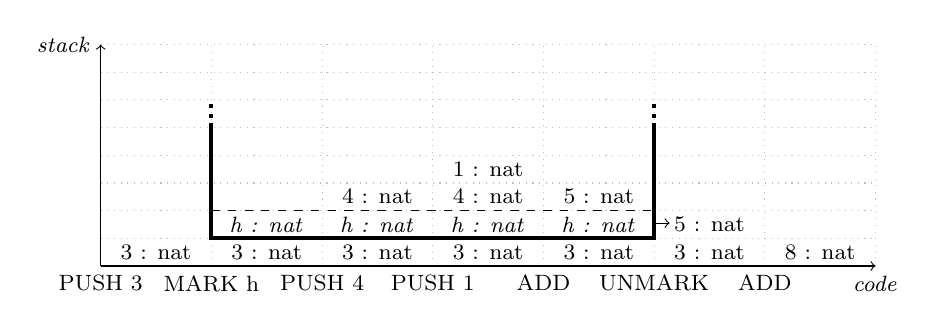
\begin{tikzpicture}[x=4em,y=1em,font=\footnotesize]
		\draw[lightgray,step=1,dotted] (0,0) grid (7,8);
		\draw[->] (0,0) -- (7,0) node[below] {\textit{code}};
		\draw[->] (0,0) -- (0,8) node[left] {\textit{stack}};

		\draw
			(0.5,0.5) node {\ident{3 : nat}}
			
			(1.5,0.5) node {\ident{3 : nat}}
			(1.5,1.5) node {\ident{\textit{h : nat}}}
			
			(2.5,0.5) node {\ident{3 : nat}}
			(2.5,1.5) node {\ident{\textit{h : nat}}}
			(2.5,2.5) node {\ident{4 : nat}}
			
			(3.5,0.5) node {\ident{3 : nat}}
			(3.5,1.5) node {\ident{\textit{h : nat}}}
			(3.5,2.5) node {\ident{4 : nat}}
			(3.5,3.5) node {\ident{1 : nat}}
			
			(4.5,0.5) node {\ident{3 : nat}}
			(4.5,1.5) node {\ident{\textit{h : nat}}}
			(4.5,2.5) node {\ident{5 : nat}}
			
			(5.5,0.5) node {\ident{3 : nat}}
			(5.5,1.5) node {\ident{5 : nat}}
			
			(6.5,0.5) node {\ident{8 : nat}}
			;
		\draw
			(0,0) node[below] {\ident{PUSH 3}}
			(1,0) node[below] {\ident{MARK h}}
			(2,0) node[below] {\ident{PUSH 4}}
			(3,0) node[below] {\ident{PUSH 1}}
			(4,0) node[below] {\ident{ADD}}
			(5,0) node[below] {\ident{UNMARK}}
			(6,0) node[below] {\ident{ADD}}
			;
		\draw[line width=1.5pt]
			(1,5) -- (1,1) -- (5,1) -- (5,5);
		\draw[line width=1.5pt,dotted]
			(1,5) -- (1,6)    (5,5) -- (5,6);
		\draw[dashed]
			(1,2) -- (5,2);
		\draw[->]
			(5,1.55) -- (5.14,1.55);
	\end{tikzpicture}
	\caption{Execution of an expression with the handler frame outlined.}
	\label{fig:stack-frames}
\end{figure}

The handler frame is delimited by the corresponding \ident{MARK} from the left,
the corresponding \ident{UNMARK} from the right, and the corresponding handler
on the stack from the bottom. Within the handler frame, evaluation of the
guarded\footnote{%
By ``guarded'' we mean that the expression is the main expression of
some catch-expression.
} expression runs independently from the context. Finally, after executing
\ident{UNMARK}, a single value is left on top of the stack: this is exactly
the denotation of the guarded expression.

Of course, handler frames may be nested since catch-expressions may also
be nested arbitrarily.
Hence, handler frames is what corresponds to catch-expressions on the operational
side of the matter.

\todo{Extended handler frames. Generalize for any expression. Exploitable for proving?
Is there some yet undiscovered direct 1:1 correspondence that would trivialize proofs?}

\subsection{Stack unwinding}
Now that handler frames are defined, we can describe exception handling
by stack unwinding quite concisely: abandon the innermost handler frame\footnote{%
Note that this involves discarding stack items but also skipping all instructions
that were to be executed within the handler frame.},
remembering the handler found at the bottom of the frame, and then
execute the handler as ordinary code on the resulting stack.

\subsection{Machine state}

As for the machine state, we discard our experiments with placeholders and return
to the original stack representation with two cons-constructors.
Instead of placeholders, we extend the state of the machine by distinguishing between
two modes of operation:
\begin{itemize}
	\item normal operation, where we just need to keep track of the stack;
	\item exception handling mode, where we keep additional state variables besides the stack.
\end{itemize}

\subsection{Differences to real machines}

In real machines, the above distinction would be represented by yet another
state variable determining which mode of operation the machine is in.
We will model it as different constructors of the \ident{State} data type.

Like in the placeholder method, we will push handlers on the stack, which
contradicts the principles we pursue and isn't really executable by real
machines. We will address this issue later, in Chapter \ref{chap:compiling2}.%
\footnote{This also causes trouble with termination but, unlike the
executability objection, termination issues can be worked around with
standard termination-proving methods or other tricks.}

For quitting the current handler frame, we need to skip all instructions
belonging to it. This is not so straightforward if we want to keep the
recursion structural. The termination checker of Agda requires that our
definitions be \emph{obviously} terminating, namely, structurally recursive,
which the following definition is not.
\begin{code}
  execCode : forall {s t} -> Code s t -> State s -> State t
  execCode nil state = state
  execCode (i <| is) state = execCode is (execInstr i state)
  execCode (THROW <| is) state = execInstr (skipToHandler is) state
\end{code}
In the snippet above, there is no single argument of \ident{execCode} that
obviously decreases in every recursive call: on the third line, the second
argument does not; on the fourth line, the first one does not -- and there
is no other argument that could possibly take the constantly-decreasing role.

There are several standard ways how to cope with this issue: accessibility
predicates, decreasing measures, or rewriting the algorithm to be
structurally recursive -- and we will aim for the last one.

This is the reason why we ``simulate'' the jump by switching the machine to an
alternative mode of execution and keep the function \ident{execCode}
structurally recursing over the instruction sequence.

Also, the type of the function \ident{execInstr}, that describes effects of
instructions on the machine state, takes only the instruction and state and
returns the new state. Since we don't include the ``instruction pointer'' in
the state, there is no way for the instructions to cause jumps in the code in
this setup without adding the special states or changing how execInstr works.

\todo{Not worse than GMH because they don't jump to addresses when looking for
the handler either; they even use implicit stacks.}

\subsection{Implementation}

The normal mode of operation contains simply the stack. However, the exceptional state
is a bit more involved; let us declare the datatypes and the auxiliary functions first
and describe them afterwards.

First, we need to know whether there is an appropriate handler on the stack and what type
it has. The shape of the stack is sufficient to determine this.
\begin{code}
  -- Get the type of the &\cident{n}&\-th top\-most handler in the Shape.
  -- Return &\cident{nothing}& if there is no such handler.
  unwindHnd : Shape -> \bN -> Maybe U
  unwindHnd (Han u :: xs) zero    = just u
  unwindHnd (Han _ :: xs) (suc n) = unwindHnd xs n
  unwindHnd (Val _ :: xs) n       = unwindHnd xs n
  unwindHnd []           _       = nothing
\end{code}

\noindent We also need to know what shape the unwound stack will have.
\label{sec:ham-unwindShape}\begin{code}
  -- Unwind the shape up to just below the &\cident{n}&\-th top\-most handler.
  -- Return the empty shape if there is no such handler.
  unwindShape : Shape -> \bN -> Shape
  unwindShape (Han _ :: xs) zero    = xs
  unwindShape (Han _ :: xs) (suc n) = unwindShape xs n
  unwindShape (Val _ :: xs) n       = unwindShape xs n
  unwindShape []           _       = []
\end{code}

\noindent Now we can define the data types. First, the resumption point, which
represents information needed to resume computation after skipping the instructions
of the current handler frame.
\begin{code}
  -- Normal operation resumption point.
  data Resume (s : Shape) : Maybe U -> Set where
    -- A handler is available, also remember the stack on which
    -- the handler should operate.
    Caught : forall {u} -> Code s (Val u :: s) -> Stack s -> Resume s (just u)
    -- Uncaught throw.
    Uncaught : Resume s nothing
\end{code}

\noindent This finally allows us to define the data type of machine states, which represents
the two operational modes of the machine: normal mode and exception-handling mode.
\begin{code}
  data State : Shape -> Set where
  	-- Normal state
  	\tick[_] : forall {s} -> Stack s -> State s
  	-- Exception\-processing state
  	\x[_,_] : forall {s : Shape}
  	  -> (n : \bN&\!&)
  	  -> Resume (unwindShape s n) (unwindHnd s n)
  	  -> State s
\end{code}

\noindent As mentioned above, the alternative \ident{\tick[\_]} represents the normal mode
of operation, where the machine just needs to keep track of the stack.

The alternative \ident{$\times$[\_,\_]} represents the exception-handling state, described by
two (explicit) parameters.
\begin{itemize}
	\item The parameter~\ident{n} describes how many handler frames we need to
		\emph{unconditionally} unwind before starting to search for an exception handler.
		
		This is needed because while skipping instructions belonging to the current
		handler frame, we might enter additional handler frames nested within. Hence
		we need to keep track of the depth of nesting.
		
		This is exactly the point where Hutton \& Wright use an implied stack.\cite[pg.~7]{gmh:exceptions}
		In their function \ident{skip}, they use the implicit call stack to count
		the nesting levels. However, we want to make this counter explicit so we include
		it as a natural number into the machine state.
		
	\item The other parameter describes how to resume normal execution when
		the machine has finished skipping instructions.
		
		If there was an appropriate handler on the stack at the time of throwing
		the exception, this parameter contains the handler and the stack obtained
		by stack unwinding. If not, the (appropriately typed) constructor
		\ident{Uncaught} indicates that an uncaught exception was thrown.
\end{itemize}

\noindent Note that the whole machinery of types ensures a great part of correctness:
\begin{itemize}
	\item of course, types of all values, handlers and expressions match;
	\item resumption points representing uncaught exceptions cannot be included in the state
		if there is a handler on the stack;
	\item vice versa, resumption points representing handled exceptions cannot be included
		in the state if there is no handler on the stack.
\end{itemize}

Also note that in spite of these non-trivial data types used to model the
machine state, it is probably obvious that in real implementations, they boil
down to just a stack and a couple of additional state variables; with the
notable exception of an arbitrarily-sized handler in the case of the
constructor \ident{Caught}, which will be addressed later.

\subsection{Operation}

Now that we know what the state \emph{looks like}, we can take a look at how it \emph{works}.
This involves redefining the function \ident{execInstr} to describe effects of instructions
in our new setting.

But first, we need to define a prerequisite for \ident{execInstr}: the function
\ident{unwindStack} that calculates a resumption record from the given stack. This record
is needed for reinstation of computation once all appropriate instructions have been skipped.

\label{sec:ham-unwindStack}\begin{code}
  unwindStack : forall {s} -> Stack s -> (n : \bN&\!&)
    -> Resume (unwindShape s n) (unwindHnd s n)
  unwindStack (h \sconsh xs) zero = Caught h xs
  unwindStack (h \sconsh xs) (suc n) = unwindStack xs n
  unwindStack (x \scons xs) n = unwindStack xs n
  unwindStack snil n = Uncaught
\end{code}

\noindent The function \ident{unwindStack}, in accordance with the functions
defined above, takes a natural number \ident{n} denoting how many handler
frames are to be thrown right away before starting a search for a handler.  If
there are no suitable handlers, the alternative \ident{Uncaught} is returned.

Now we can proceed to the definition of the functions \ident{execInstr} and
\ident{execCode}, this time in a \ident{mutual} block.

\begin{codei}
  mutual
    execInstr : forall {s t} -> Instr s t -> State s -> State t
  	-- Normal operation
    execInstr ADD 			\tick[ x \scons y \scons st ]	= \tick[ (x + y) \scons st ]
    execInstr (PUSH x)		\tick[ st ] 		= \tick[ x \scons st ]
    execInstr (MARK h)		\tick[ st ] 		= \tick[ h \sconsh st ]
    execInstr UNMARK		\tick[ x \scons h \sconsh st ]	= \tick[ x \scons st ]
    -- Exception throwing  
    execInstr THROW			\tick[ st ] = \x[ zero , unwindStack st zero ] 
    -- Nontrivial exception processing
    execInstr (MARK _)		\x[ n	 ,	r	] = \x[ suc n, r ]
    execInstr UNMARK		\x[ suc n ,	r	] = \x[ n	, r ]
    execInstr UNMARK		\x[ zero	 , Caught h st	] = execCode h \tick[ st ]
    -- Trivial exception processing: instruction skipping
    execInstr THROW			\x[ n , r ] = \x[ n , r ]
    execInstr ADD			\x[ n , r ] = \x[ n , r ]
    execInstr (PUSH _)		\x[ n , r ] = \x[ n , r ]
\end{codei}
\begin{code}
    -- Code execution is still a left fold over instructions.
    execCode : forall {s t} -> Code s t -> State s -> State t
    execCode \nil st = st
    execCode (i <| is) st = execCode is (execInstr i st)
\end{code}

\noindent The above definition of the function \ident{execInstr} is mostly
straightforward.  First, we deal with the normal state, defining how it changes
when different instructions are executed.

The first block is essentially equivalent to what we defined for the
placeholder method in \Fref{sec:placeholder}.

Then we define what effect the instruction \ident{THROW} has. The two actions
that constitute stack unwinding (\Fref{sec:stack-unwinding}) are
represented as follows:

\begin{itemize}
	\item Popping items from the stack until a handler is found is done by the
		function \ident{unwindStack}. If a handler is found, it is returned
		along with the unwound stack as an instance of the constructor
		\ident{Caught}. Otherwise, an instance of the constructor
		\ident{Uncaught} is returned.
		The result of the function \ident{unwindStack} is then stored in the
		state of the machine.

	\item Skipping instructions that belong to the handler frame is done by
		switching the machine to the instruction-skipping state. The state also
		contains a natural number that keeps track of nesting depth of handler
		frames along the way (see the next paragraph for a more detailed
		description). This value is initially zero.
\end{itemize}

The reason why we need to keep track of the nesting depth is that instruction
skipping always ends at an \ident{UNMARK} instruction -- but not always the
first one encountered. The instruction sequence we want to skip may contain
more \ident{MARK}-\ident{UNMARK} pairs if the current handler frame contains
more nested handler frames. Hence we need to count \ident{MARK}s along the way
and then skip that number of \ident{UNMARK}s before stopping at the real
\ident{UNMARK} we are looking for.

Next, we define the core part of exception processing: dealing with the
instructions \ident{MARK} and \ident{UNMARK}.

In the exception-processing mode, the effect of the instruction \ident{MARK} is
quite trivial: it just increments the handler frame nesting counter contained
in the state.

If the frame nesting counter is nonzero, then the effect of the instruction
\ident{UNMARK} is trivial, too; it just \emph{decrements} the frame nesting
handler.

However, if the frame nesting counter is zero, the effect of the instruction
\ident{UNMARK} is a bit more complex: it can be described as switching the
machine to the normal mode using the saved stack, and then running the
saved exception handler.

This is exactly the point where we use the resumption record to reinstate
normal operation after having skipped all instructions that were to be skipped.

Note that in the non-trivial case for the instruction \ident{UNMARK}, we know
for sure that the state contains an instance of the \ident{Caught} constructor%
\footnote{As opposed to an instance of the \ident{Uncaught} constructor.}, so
we can be always sure there is a saved handler and stack available for
exception handling. The other option is simply ruled out by the type of the
stack: we are executing \ident{UNMARK}, whose type indicates that a handler
must be available.\footnote{To be explicit, because the type indices of the
	instruction \ident{UNMARK} and of the current state must match, the shape
	of the current state must contain a value \ident{Han u} for some \ident{u}
	as the second-to-top item.  This prevents the function \ident{unwindHnd}
from returning \ident{nothing}, but since \ident{nothing} is exactly the index
of \ident{Uncaught}, this constructor cannot occur in this situation.} This all
is understood by Agda and this pattern coverage is accepted as complete.

Finaly, we conclude our definition of the function \ident{execInstr} by
defining that in the exception-handling mode, all other instructions are not
interesting and they should be simply skipped without having any effect on the
machine state.

Note that, unlike in the placeholder method, there is only one case for each
such ``uninteresting'' instruction causing the machine to simply skip it, as
opposed to $2^{\mathrm{arity(instr)}} - 1$ cases in the placeholder method,
where we had to account for every possible combination of placeholders on the
stack. We have reduced both the number of cases, and their complexity.

Also note that in the whole specification, there are no implicit stacks: our
functions are completely tail-recursive. We designed the machine to work this
way to meet our requirements from the Introduction (page~\pageref{objectives}).

Both modes of execution are essentially the same; both contain stack, the
exception-handling mode also contains a number and a saved exception handler.
Thus only the arbitrarily-sized handler violates our simplicity requirement.
We will deal with this issue later in the Chapter \ref{chap:compiling2}.

\subsection{Termination}

However, this solution has a serious flaw: it is not structurally recursive.
As already mentioned, Agda will accept only definitions that are \emph{obviously}
terminating but the pair of functions \ident{execInstr} and \ident{execCode}
is not.

The apparent culprit is the call of \ident{execCode} from within
\ident{execInstr} in the non-trivial, exception-handling case for
\ident{UNMARK}. The function \ident{execCode} recurses structurally over its
first (explicit) argument, the code sequence. However, the handler that is to
be executed is not structurally smaller than the code sequence where the
\ident{UNMARK} came from, let alone \emph{obviously} structurally smaller.

There are several ways of coping with this issue, as already mentioned.

First, we can resign on naturally structural recursion altogether and, instead,
use the pen-and-paper-like termination proving method: a decreasing measure.
This approach is quite straightforward and although it works and offers no
surprises, it is tedious and inelegant.

Second, we could exploit a deeper insight in how our high-level and low-level
languages are connected and define an intermediate data structure that would
facilitate showing correspondence between the two.%
\footnote{In combination with this approach, the Bove-Capretta method can be used to
extract termination proof obligations from the code, in order to separate the
informative part and the termination proof, neither cluttering code with
proofs, nor proofs with too much information.} Such a connection would probably
be useful in proving correctness of the compiler, too.

\todo{Insert a reference to the Bove-Capretta paper wherever it appears.}

For example, note that any \emph{guarded expression} is
``transactional'', in the sense that if it fails, all traces of its execution
are cleared up and the handler code is run instead. When considering just
effects of the code, it appears that in every handler frame, either the regular
code is (completely) executed or the handler code is (completely) executed,
which creates a ''fork'' of possible execution scenarios at the entrypoint of
each handler frame -- and this can be modelled using a suitable data structure.

However, while it looks promising and the transformation of code to the
``forking'' data structure is not too complicated, the author has not been able
to prove termination using this approach. This might be an interesting direction
for further research.

Third, we can try hard and make the recursion structural. As already hinted,
this is the approach we prefer to take in this thesis and we will develop it
further in \Fref{sec:handlers-at-unmark}.

\subsection{Compared to the placeholder method}

So what about the objections we raised when evaluating the placeholder method
in \Fref{sec:placeholders-objections}?

First, our current low-level language is no longer a trivial model of how the
denotation function \ident{denExp} gets evaluated and its execution is closer
to how real machines work.

Second, handling exceptions uses a different mechanism than actually executing
every instruction. In the exception-handling mode, (non-interesting)
instructions are skipped without much fuss: there is only one case per
instruction, compared to $2^\mathrm{arity}$ in the placeholder
case.\footnote{Theoretically, we could even do better and replace all trivial
cases with the wildcard pattern \ident{\_}. However, if we do that, Agda will
complain because it cannot check that the types involved are correct
-- they are slightly different across different cases and they need to be
checked separately.}

Third, actual efficiency of the pattern match is comparable to that of the
placeholder method. We actually cannot do better than going through every
single instruction if we want to recurse structurally over \ident{code}.
However, the work we do at every instruction in the exception-handling mode is
trivial: we simply skip it. No stack inspection, no manipulation with machine
state at all.  Hence, when entering the exception handling mode, the machine
focuses just on the code sequence and starts to search an appropriate place to
resume execution at. This approximates real-world jumps better although we still
need to keep track of what instruction is being skipped and when we need to
stop skipping.

Fourth, unfortunately, our recursion is still not structural and the
termination checker rejects the recursive call to \ident{execCode} in the
handler-running clause of \ident{execInstr}. However, we are going to address
this shortcoming soon in the next sections.

\todo{Which sections? Insert references.}

Fifth, we still keep pushing blobs of code on the stack so we haven't improved
this aspect yet -- but we are going to as well, in later sections.

\todo{Which sections? Insert references.}

\subsection{Remarks}

It is worth noting that the expression \ident{Throw} is indexed as an expression
that yields a value of \emph{any} type, and the instruction \ident{THROW} is indexed
as if it pushed a value of any type on the stack -- without actually having a value
of that type (which would be of course impossible if it was the empty type).

This resembles exceptions in typed functional languages; for example the function
\ident{throw} in Haskell:
\begin{code}
  throw :: Exception e => e -> a
\end{code}
The function \ident{throw} can ``promise'' to yield a value of any type because,
in fact, it never returns. In a way, it behaves as \emph{bottom}.

Finally, we don't prove correctness of this implementation because we don't
have a proof of termination and since we are going to fix that soon, let us
leave it that way.

\section{Execution: handlers at \ident{UNMARK}}
\label{sec:handlers-at-unmark}

Our (non-)termination trouble arises from the fact that before running an
exception handler, we move it around, push it on the stack, run other code, pop
it from the stack etc., which obscures the fact that we never execute the same
instruction twice.

Instead of partitioning the code at runtime, shuffling the partitions and
executing them in a different order, it is better to already \emph{generate}
the code in a more convenient way.

A surprisingly simple change solves all the terminating trouble: let us just
attach handler code to the instruction \ident{UNMARK} instead of the
corresponding \ident{MARK}.

\subsection{Virtual machine}

First, we alter the definition of the type of instructions from
\Fref{sec:gmh-ham-instr} a bit -- we make the \ident{UNMARK} constructor take
the exception handler instead of the \ident{MARK} constructor.

\begin{code}
  data Instr : Shape -> Shape -> Set where
    PUSH : forall {u s} -> el u -> Instr s (Val u :: s)
    ADD : forall {s} -> Instr (Val nat :: Val nat :: s) (Val nat :: s)
    MARK : forall {u s} -> Instr s (Han u :: s)
    UNMARK : forall {u s} -> Code s (Val u :: s) -> Instr (Val u :: Han u :: s) (Val u :: s)
    THROW : forall {u s} -> Instr s (Val u :: s)
\end{code}

Second, we also need to alter the type of stacks from \Fref{sec:gmh-ham-stack}
because we will no longer push handlers on the stack. However, we want to
preserve the overall principle of execution so we have to push \emph{something}
to keep the stack well-typed.  Hence, we will push a placeholder\footnote{ Note
that this placeholder is different from the one used in the placeholder
execution method, where we pushed bogus \emph{values}, not handlers.} instead
of code, indicating that a handler can be found at the appropriate
\ident{UNMARK}.

\begin{code}
  infixr 50 _\scons\_
  infixr 50 \void\sconsh\_
  data Stack : Shape -> Set where
    snil : Stack []
    _\scons\_ : forall {u s} -> el u -> Stack s -> Stack (Val u :: s)
    \void\sconsh\_ : forall {u s} -> Stack s -> Stack (Han u :: s)
\end{code}

\subsection{Compiler}

We will make just the small obvious change in the compiler from
\Fref{sec:gmh-ham-compile}: move the compiled handler from \ident{MARK} to \ident{UNMARK}.

\label{sec:hau-compile}\begin{code}
compile : forall {u s} -> Exp u -> Code s (Val u :: s)
compile (Lit x) = [[ PUSH x ]]
compile (Bin op l r) = compile r \app compile l \app [[ opInstr op ]] 
compile Throw = [[ THROW ]]
compile (Catch e h) = [[ MARK ]] \app compile e \app [[ UNMARK (compile h) ]]
\end{code}

\subsection{Machine state}

With this approach, machine state is simplified quite a lot. There are no
resumption records and both execution modes contain just the stack (augmented
with a nesting counter in the exception-handling case).

\begin{code}
  data State (s : Shape) : Set where
    \tick[_] : Stack s -> Shape s
    \x[_,_] : (n : Nat&\!&) -> Stack (unwindShape s n) -> State s
\end{code}

\subsection{Execution}

Execution is simplified as well.  Suddenly, recursion is naturally completely
structural. In the following code, we will use the auxiliary functions
\ident{unwindShape} (\Fref{sec:ham-unwindShape}) and \ident{unwindStack}
(\Fref{sec:ham-unwindStack}), trivially modified to work with the stack type we
are using here.

\begin{codei}
  mutual
    execInstr : forall {s t} -> Instr s t -> State s -> State t
  	-- Normal operation
    execInstr ADD 				\tick[ x \scons y \scons st ]	= \tick[ (x + y) \scons st ]
    execInstr (PUSH x)			\tick[ st ] 		= \tick[ x \scons st ]
    execInstr MARK				\tick[ st ] 		= \tick[ \void\sconsh st ]
    execInstr (UNMARK _)		\tick[ x \scons \void\sconsh st ]	= \tick[ x \scons st ]
    -- Exception throwing  
    execInstr THROW				\tick[ st ] = \x[ zero , unwindStack st zero ] 
    -- Nontrivial exception processing
    execInstr MARK				\x[ n	 , st	] = \x[ suc n, st ]
    execInstr (UNMARK _)		\x[ suc n , st	] = \x[ n	, st ]
    execInstr (UNMARK h)		\x[ zero	 , st	] = execCode h \tick[ st ]
    -- Trivial exception processing: instruction skipping
    execInstr THROW			\x[ n , st ] = \x[ n , st ]
    execInstr ADD			\x[ n , st ] = \x[ n , st ]
    execInstr (PUSH _)		\x[ n , st ] = \x[ n , st ]
\end{codei}
\begin{code}
    -- Code execution is still a left fold over instructions.
    execCode : forall {s t} -> Code s t -> State s -> State t
    execCode \nil st = st
    execCode (i <| is) st = execCode is (execInstr i st)
\end{code}

\noindent Note that:
\begin{itemize}
	\item the $\times[\_]$ constructor now takes only the (unwound) stack, nothing more;
	\item in the third and fourth clause of the function \ident{execInstr},
		we push and pop only placeholders instead of exception handlers;
	\item in the eighth clause, we call \ident{execCode} recursively; this time however,
		the code argument \ident{h} is \emph{structurally smaller} than that of
		the (grand-)parent call to \ident{execCode}. Agda recognizes this and
		accepts our definition without complaining.
\end{itemize}
This is actually all it takes to make execution work with this approach.

\subsection{Correctness}

Since we have eliminated the termination trouble, we can proceed to proving
correctness. We do this by induction on the given expression, in a way
very similar to how the proof was done in \Fref{sec:cor-correctness}, using
equational reasoning.

\todo{Insert a reference to the source code.} The complete proof can be found
in the attached code; here we will just outline the main theorem and the
accompanying lemmas.

The theorem has almost the same shape as before in \Fref{sec:cor-correctness},
namely:
\begin{code}
  correctness : forall {u} (e : Exp u) (s : Shape) (st : State s)
    -> execCode (compile e) st == (denExp e ::: st)
\end{code}\label{sec:hau-correctness}

\noindent This time, we don't prove the correctness with any \emph{stack} but
with any \emph{state}, which is more useful in the proof (especially when
using the induction hypothesis).

The operator \ident{:::} is the ``smart stack pusher'' that pushes values
to the stack contained within a state, dealing correctly with all combinations
of cases that may occur; for example, the denotation function \ident{denExp}
may return \ident{nothing} and the state \ident{st} may be in the process
of handling an exception.

\begin{codei}
  infixr 5 _:::_
  _:::_ : forall {u s} -> Maybe (el u) -> State s -> State (Val u :: s)
  just x	:::	\tick[ st ]		= \tick[ x \scons st ]
  nothing	:::	\tick[ st ]		= \x[ zero , unwindStack st zero ]
  just x	:::	\x[ n , st ]	= \x[ n , st ]
  nothing	:::	\x[ n , st ]	= \x[ n , st ]
\end{codei}

\noindent The use of this operator makes our theorems quite neat and concise.

As already mentioned, we prove this correctness theorem by induction on the
expression \ident{e}

The first lemma we use is the distributivity lemma; again, practically
identical to that in \Fref{sec:cor-compile-distr}.
\begin{code}
  distr : forall {s t u} (st : State s) (c : Code s t) (d : Code t u)
    -> execCode (c \app d) st == (execCode d \o execCode c) st
\end{code}

We also use two lemmas that perform specialized case analysis. When doing
induction on the structure of the expression while proving correctness, there
are two non-trivial cases: the case of binary operators\footnote{The
constructor \ident{Bin}.} and the case of catch-expressions\footnote{The
constructor \ident{Catch}.}. Apart from containing sub-expressions recursively
(thus requiring the induction hypothesis), it is non-trivial to show that the
effect of the code compiled from these expressions conforms to their
denotational semantics with respect to exception propagation.  This is where we
use the two lemmas to analyze all these cases, one for the constructor
\ident{Bin}, the other for the constructor \ident{Catch}.

\begin{code}
  lemma\-op : forall {s t u v} (r : Exp t) (l : Exp u) (op : Op u t v) (st : State s)
    -> execInstr (opInstr op) (denExp l ::: denExp r ::: st)
      == denExp (Bin op l r) ::: st
\end{code}

\begin{code}
  lemma\-catch : forall {s u} (e : Exp u) (h : Exp u) (st : State s)
    -> (forall {s} (st' : State s) -> execCode (compile h) st' == denExp h ::: st')
    -> execInstr (UNMARK (compile h)) (denExp e ::: execInstr MARK st)
      == denExp (Catch e h) ::: st
\end{code}

The lemma \ident{lemma-catch} also takes the induction hypothesis as an
argument, instantiated for the compiled handler code.

This is all we need to prove correctness (as stated in
\Fref{sec:hau-correctness}): the cases for the constructors \ident{Throw} and
\ident{Lit} can be trivially discharged using \ident{refl}; the cases for the
constructors \ident{Bin} and \ident{Catch} are proved equationally, using the
above lemmas.

\subsection{Remarks}

We have solved the fourth objection introduced in
\Fref{sec:placeholders-objections}: recursion is now structural, termination
follows trivially from this fact and need not be proved explicitly.

What's left is the fifth problem related to pushing code blobs on the stack.
This is solved by linearizing handlers in the main code sequence and adding
jumps so that these handlers are skipped unless actually needed.

\section{Linearized code}

% tra tra tra




























































